\documentclass[10pt,xcolor=table ]{beamer}
	
\usetheme{metropolis}
\usepackage{appendixnumberbeamer}

\usepackage{booktabs}
\usepackage[scale=2]{ccicons}

\usepackage{pgfplots}
\usepgfplotslibrary{dateplot}

\usepackage{xspace}
\usepackage{graphicx}
\usepackage{graphics}


\usepackage[spanish]{babel}
\usepackage[utf8]{inputenc}

\usepackage{decorule}
\newcommand{\decoRule}{\rule{\textwidth}{.4pt}} % New command for a rule to be used under figures


\usepackage{pgf-pie}
\usepackage{pgfplots}

\usepackage[export]{adjustbox}


\definecolor{UniBlue}{RGB}{255,255,255}
\setbeamercolor{background canvas}{bg=UniBlue}


\begin{document}

\maketitle

\subsection{Diseño de cursos y programas}
\begin{frame}{Diseño de cursos y programas}
	\begin{figure}
		\centering
	    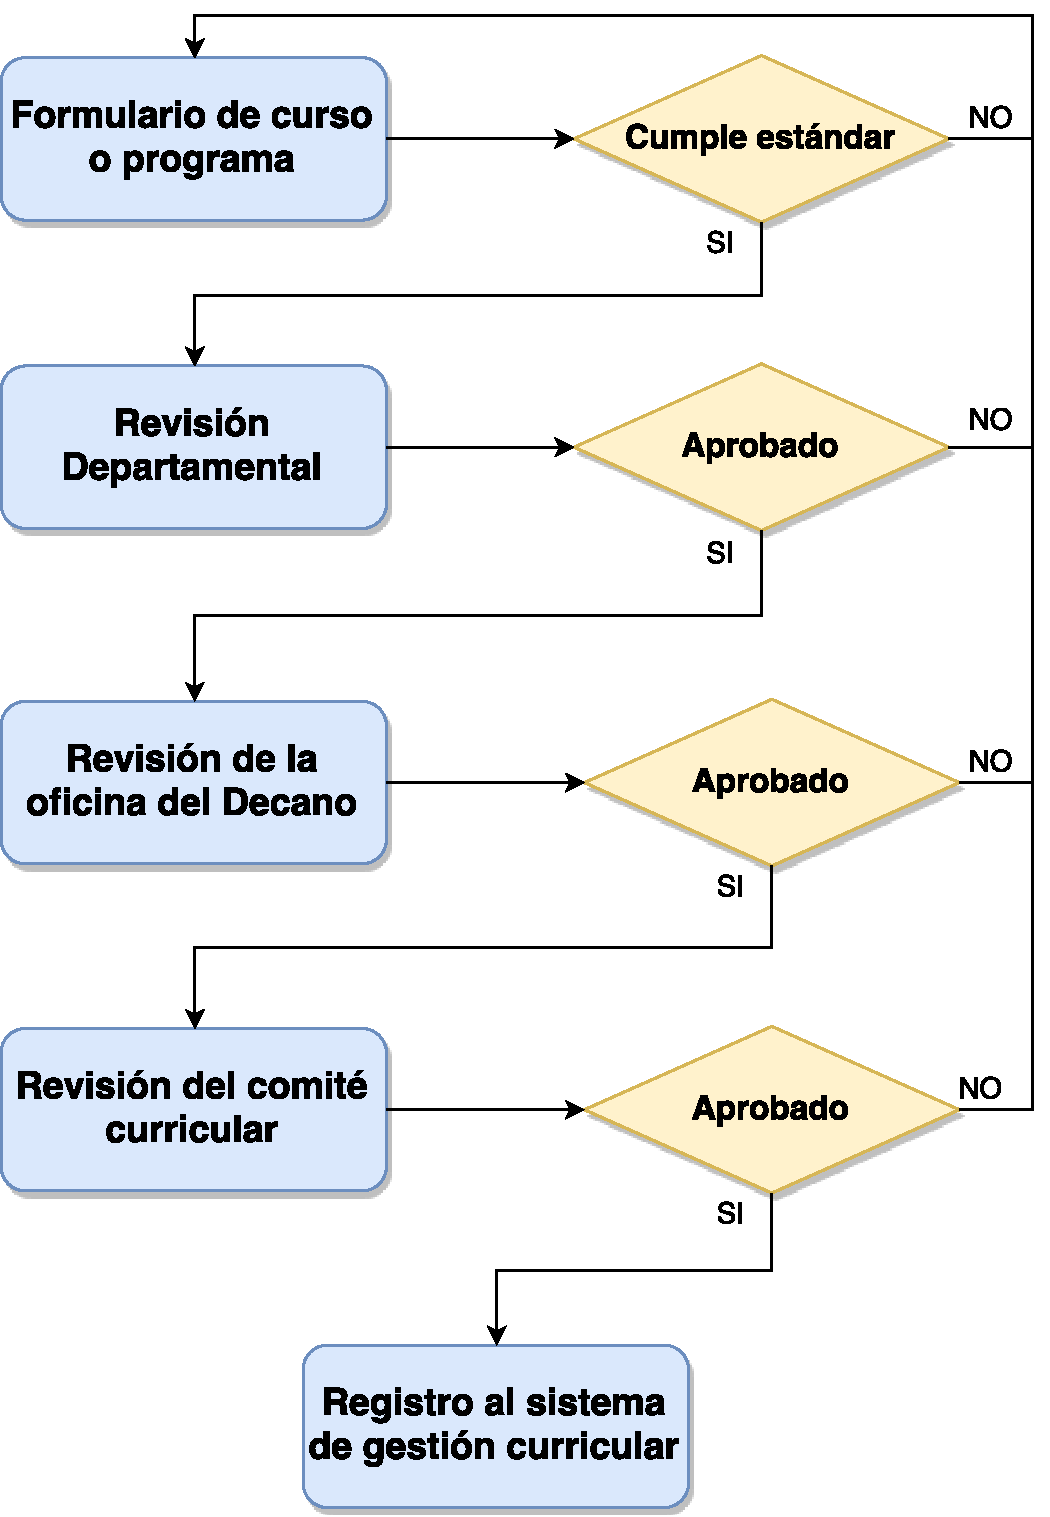
\includegraphics[scale=0.3]{../Figuras/course_creation_flow}
	\end{figure}
\end{frame}


\end{document}
